\documentclass[tikz,border=8pt]{standalone}
\usepackage{amsmath}
\usetikzlibrary{arrows.meta,decorations.pathreplacing}
\begin{document}

% Asset ID: AS2DataPresentationTikZ-007
% Source: Frequency polygon evidence.
% Related lesson section: Core Theory, Frequency Polygons.
% Purpose: Form a frequency polygon by joining histogram bar midpoints.
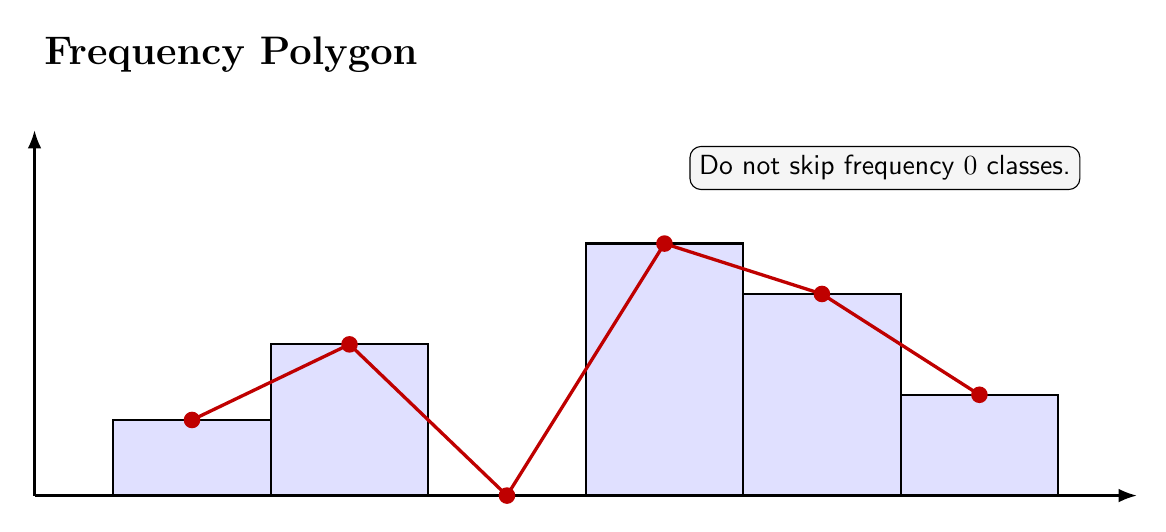
\begin{tikzpicture}[x=1cm,y=0.08cm,>=Latex,font=\sffamily]
\node[anchor=west,font=\bfseries\Large] at (0,70){Frequency Polygon};
\draw[->,thick] (0,0)--(14,0); \draw[->,thick] (0,0)--(0,58);
\draw[fill=blue!12,thick] (1,0) rectangle (3,12); \draw[fill=blue!12,thick] (3,0) rectangle (5,24); \draw[fill=blue!12,thick] (5,0) rectangle (7,0); \draw[fill=blue!12,thick] (7,0) rectangle (9,40); \draw[fill=blue!12,thick] (9,0) rectangle (11,32); \draw[fill=blue!12,thick] (11,0) rectangle (13,16);
\draw[very thick,red!75!black] (2,12)--(4,24)--(6,0)--(8,40)--(10,32)--(12,16);
\foreach \x/\y in {2/12,4/24,6/0,8/40,10/32,12/16}{\fill[red!75!black] (\x,\y) circle (3pt);}
\node[draw,rounded corners,fill=gray!8,align=center] at (10.8,52){Do not skip frequency $0$ classes.};
\end{tikzpicture}

\end{document}
